\documentclass[10pt, a4paper]{article}

\usepackage{amsmath}
\usepackage{amssymb}
\usepackage{fullpage}
\usepackage{algorithm2e}
\usepackage{graphicx}
\usepackage{wrapfig}



\newcounter{wssection}
\newcounter{wsexercise}[wssection]


\newcommand{\worksheetsection}[1]{
\vspace{10mm}
\stepcounter{wssection}
\noindent \Large \textbf{\thewssection. #1} \normalsize
\vspace{3mm}
}


\newcommand{\worksheetexercise}{
\stepcounter{wsexercise}
\vspace{5mm} \noindent \textbf{Exercise \thewssection.\thewsexercise \;}
}


\title{Dublin R Workshop on Bayesian Data Analysis}
\author{Mick Cooney\\mickcooney@gmail.com}
\date{July 29, 2013}



\begin{document}

\maketitle


\worksheetsection{Conditional Probability}

\noindent
Suppose that in the general population, the probability of having a
specific rare disease (the Dreaded Lurgy) is one in a thousand. We
denote the true presence or absence of the disease as the value of a
parameter, $\theta$, that can have the value 1 if disease is present,
or the value 0 if the disease is absent. The base rate of the disease
is therefore denoted $p(\theta = 1) = 0.001$. This is our prior belief
that a person selected at random has the disease.

Suppose that there is a test for the disease that has a 99\% hit rate,
which means that if a person has the disease, then the test result is
positive 99\% of the time. We denote a positive test result as $D = 1$,
and a negative test result as $D = 0$. The observed test result is
a bit of data that we will use to modify our belief about the value of
the underlying disease parameter. The hit rate is expressed as
$p(D = 1 \, | \, \theta = 1) = 0.99$.

The test also has a false alarm rate of 5\%. This means that 5\% of
the time when the disease is not present, the test falsely indicates
that the disease is present. Wedenote the false alarm rate as
$p(D = 1 \, | \, \theta = 0) = 0.05$.

However, what we need to know is $p(\theta = 1 \, | \, D = 1)$, i.e. the
probability that the patient has the disease given a positive test
result.

We can calculate the above conditional probability given Bayes' Rule
and a bit of arithmetic and algebra, and, somewhat
counter-intuitively, it says the probability is slightly below 2\%.

We will try to estimate this probability using simulation.

\worksheetexercise
The supplied function \texttt{generate.disease.test.data()} generates
sample data based on the above numbers. Look at the function
definition to see how it is used, and generate some sample data, then
use this data to estimate the conditional probability. with a
reasonable number of datapoints (say 1,000,000) you should get an
estimate close to the analytic answer.


\worksheetexercise
Why is this conditional probability so low? Experiment with the
dependency of this probability on the three input probabilities.

(Any plotting system will work, though I will use ggplot2 for mine)


\worksheetexercise
How are the probabilities changed if two independant tests are
tried. The provided function \texttt{generate.disease.twotest.data()}
generates random data for this. Using this function, calculate the
conditional probabilities of having the disease, given the various
combinations of test results.



\worksheetsection{Analytical Approach}

\noindent
Bayesian reasoning is as old as the concept of probabilities, but has
only recently started to receive a lot of attention. One likely reason
for this is that, apart from a few special cases, it is mot possible
to perform the calculations analytically.

In our application we have a prior distribution for our beliefs,
$p(\theta)$, and a likelihood for the data, $p(D | \theta)$, and
through use of the Chain Rule, we get the posterior distribution,
$p(\theta | D)$,

\[ p(\theta | D) = \int d\theta \, p(D | \theta) \, p(\theta).  \]

In those special cases, the likelihood function has a prior and
posterior distribution with the same functional form, i.e. the prior
and the posterior are two members of the same `family' of functions.

For the rest of this workshop we are going to deal with estimating the
fairness of a coin, based on the result of multiple coin tosses. We
define `success' as the toss coming up Heads, and denote this
probability as $\theta$. Thus,

\[ P(y = 1 | \theta) = \theta \hspace{5mm} \text{and} \hspace{5mm}
   P(y = 0 | \theta) = 1 - \theta. \]

\noindent
We can combine the above two into a single expression:

\[ P(y | \theta) = \theta^y (1 - \theta)^{(1 - y)} \].

Now we consider the data $y$ to be fixed, and consider the above as a
function of $\theta$. With this approach we call the above equation
\emph{the likelihood function of $\theta$}.

The Bernoulli function has a conjugate prior: the \emph{Beta}
distribution, $B(a, b)$. R supports the beta distribution natively,
via the standard grouping of functions for probability distributions:
\texttt{rbeta()}, \texttt{dbeta()}, \texttt{pbeta()}, \texttt{qbeta()}.


\worksheetexercise
Plot the density distribution for the Beta distribution using various
combinations of parameters $a$ and $b$.


\worksheetexercise
Load the data in \texttt{cointoss10}, and use it and the beta
distribution to investigate the effect of the prior on the posterior
distribution.


\worksheetexercise
Load the data in \texttt{cointoss1000}, and use it and the same priors
used in the previous exercise to investigate the effect of the prior
on the posterior distribution.


\worksheetexercise
Compare the posterior distributions for the same priors using the two
datasets. How do they compare, and why do you think this is?



\worksheetsection{Numerical Solutions using a Discrete Grid}

\noindent
For many applications, the use of simple conjugate priors is not
appropriate, and we need to deal with the posterior integral
calculation itself. Since analytical solutions do not exist, we use
numerical techniques to approximate the integral.

The supplied functions \texttt{calculate.\-data.\-probability()} and
\texttt{calculate.\-posterior.\-probability()} perform these
calculations. The major benefit of this approach is that we can now
use arbitrary priors.


\worksheetexercise
Using the \texttt{cointoss10} data, and a $B(1, 1)$ prior, use the
grid approximation to the integral to calculate the posterior
density. Compare the output of this to the analytical solution


\worksheetexercise
Repeat the previous exercise of comparing the influence of priors on
the posterior density for both the 10 coin toss and 1,000 coin toss
data. Match this output to the analytics solutions you derived
earlier.


\worksheetexercise
Suppose we think the coin has a 3/1 bias, but we do not know for which
side. Create a prior that represents this and investigate the
posterior for both sets of data.


\worksheetexercise
Estimate the posterior density for the bias in the coin assuming you
have an equally weighted prior belief of the coin being fair, or
biased 3/1 for either side.


\worksheetexercise
Investigate the influence of the size of the dataset on the posterior
for arbitrary priors.


\worksheetsection{Introducing Monte Carlo Sampling}

\noindent
The numerical integration approach works fine when the dimensionality
of the problem is low, but quickly becomes infeasible computationally
once we add start adding more parameters to the problem.

In these cases, we instead look for ways in which we can use
simulation to approximate the integral, only calculating the integral
at places on the grid where there is a significant contribution to the
solution.

For these sampling techniques, we first look at the Metropolis
algorithm:

\vspace{5mm}
\noindent
\fbox{
\begin{algorithm}[H]
Initialise $\textbf{x}_0$\;
Set $i = 1$\;
\While{$i < \text{SampleSize}$}{
    Choose new $\textbf{x}_i$\;

    \eIf{$p(\textbf{x}_i) > p(\textbf{x}_{i-1})$}{
        Accept $\textbf{x}_i$\;
    }{
        Accept $\textbf{x}_i$ with
        probability $\frac{p(\textbf{x}_i)}{p(\textbf{x}_{i-1})}$\;
    }

    Increment $i$\;
}
\end{algorithm}
}
\vspace{5mm}

Once again, we will work with a very simple example, and build up from
there.

Suppose we have a politician who is seeking election. He wants to
visit remote islands, spending time on each island in proportion with
their population. He does not know these population figures in
advance, but he knows that the locals do. To make things simple, we
will assume the islands are in a long chain, so you can only move to
an adjacent island.

If he follows the Metropolis algorithm, using the population ratios as
his probabilities, and hops from island to island, in the long run he
will visit each island in rough proportion to their population.

\worksheetexercise Using the supplied function
\texttt{do.metropolis.island.sampling()}, generate a 1000 datapoint
sample for the politician based on a four island chain where the
islands have all equal population.

\worksheetexercise Think about ways in which you might verify that the
sample is a reasonable sample from the target distribution.

\worksheetexercise Suppose we have a seven-island chain, where each
island has population proportional to its number. Sample from this
distribution using our code. Check that the sample is reasonable.

\worksheetexercise Re-run the above code with the
\texttt{proposal.prob} parameter set to 0.7. With this value, the
algorithm is more likely to propose moving to islands further up the
chain. Is there any difference in the samples from previously?

\worksheetexercise Now set the parameter to 0.3. Does the sample
output change qualitatively?

\worksheetexercise Think about what the consequences of the choice of
this parameter value.

\worksheetexercise Redo all of the above exercises, but generating a
dataset of size 10,000 datapoints. Investigate what implications exist
for sampling larger datasets.


\worksheetsection{Introducing Hierarchical Models}

\noindent
We can now extend this idea by using a hierarchical model. Previously,
we were considering the coin by itself, and the goal was to estimate
the parameters of the model. We could extend that model by using
multiple coins, but our initial intuition would be to treat multiple
coins as being independent of one another.

\begin{figure}[h]
\begin{center}
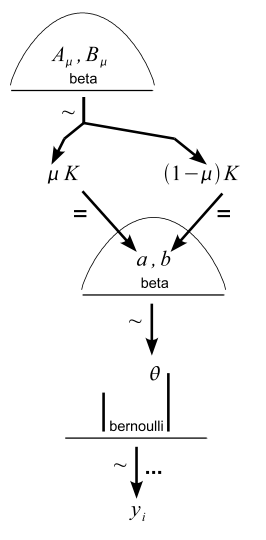
\includegraphics{hierarchical_singlemint_singlecoin.png}
\caption{\label{fig1}
Graphical Representation of the Single Mint, Single Coin
Hierarchical model}
\end{center}
\end{figure}


However, what if we were instead to also consider the fact that a coin
is minted, and the bias of the coin is probably influenced by the
manufacturing processes and quality of its origin. In this case, we
could incorporate prior beliefs about the mint as well the coin, and
then use our data to update those beliefs.

To start with, we will work from a single coin coming from a single
mint. Each coin is produced with a bias of $\theta$, but these are
also random variables drawn from another Beta distribution with mean
$\mu$. This means that outcomes of the coin tosses, $y$, are the
result of a hierarchical random process. At the top, we have a
distribution for $\mu$, and we call this the
\emph{hyperdistribution}. Accordingly, $\mu$ is a
\emph{hyperparameter}. We then use the values of the hyperparameters
as inputs to the distribution for $theta$. In turn, with the values of
$\theta$, we then determine values for the data, $y$. A graphical
representation of this model is shown in Figure \ref{fig1}.

So, the hyperparameter $\mu$ is used to determine values $A_\mu$, and
$B_\mu$ for the hyper-beta-distribution. To do this, we also need a
value $K$, which for the moment we will assume is a constant, and is a
representation of how closely the value of $\theta$ depends on
$\mu$. For high values of $K$, $\theta$ will cluster tightly around
$\mu$.

Expressing this formally, we have

\[ p(y|\theta) = \theta^y (1 - \theta)^{(1-y)} , \]

\noindent
just like before, but we now also have $\theta$ as a random variate,

\[ p(\theta | \mu) = \text{beta}(\theta | \mu K, (1 - \mu) K) \]

\noindent
with $\mu$ itself being drawn from a hyperdistribution (in this case, the
beta distribution):

\[ \mu \backsim \text{beta}(A_\mu, B_\mu). \]

Note that this model will required values for $A_\mu$ and $B_\mu$, and
these will reflect our prior beliefs about the mint. For this, we will
probably just use low constant values, representing weak prior beliefs
on the mint itself.

So, the above seems like a very interesting approach, but how do we go
about implementing the approach? It is unlikely that an analytic
solution would be either tractable or practical, but like the drunk
looking for his keys, this is where the light is.

So, we know from Bayes' Rule that

\[ p(\theta, \mu | y) = \frac{p(y | \theta, \mu) p(\theta, \mu)}{p(y)}. \]

\noindent
From our model, we can see that, conditional on $\theta$, the
likelihood model does not depend on $\mu$, and so we have

\[ p(y | \theta, \mu) = p(y | \theta). \]

\noindent
Also, from another application of Bayes' Rule,

\[ p(\theta | \mu) = \frac{p(\theta, \mu)}{p(\mu)} \implies
p(\theta, \mu) = p(\theta | \mu) p(\mu) \],

\noindent
resulting in the following expression for the posterior distribution

\[ p(\mu, \theta | y) = p(y | \theta) p(\theta | \mu) p(\mu) / p(y) \]



So, if we create a grid for both $\theta$ and $\mu$, we can
approximate the posterior from numerical integration. We take our
models for $p(y|\theta)$, $p(\theta|\mu)$ and $p(\mu)$, and create our
posterior by integration.

\worksheetexercise Use a very weak prior for $\mu$, but a value of 5
for $K$, and generate the posterior density for this model using the
\texttt{cointoss10} data. You can use the supplied function
\texttt{calculate.\-hierarchical.\-posterior()} to do this. How would you
visualise this output in a meaningful way?

\worksheetexercise How does the data affect the posterior distribution
for $\mu$ and $\theta$?

\worksheetexercise Repeat the above exercise but with a $K$ value of
100. Do you notice a difference in the posterior distributions of
$\mu$ and $\theta$?

\worksheetexercise Repeat the above for $K = 1,000$. How are the
posterior densities affected now?

\worksheetexercise Repeat all of the above using the
\texttt{cointoss1000} data.

\worksheetexercise What impact does the size of the dataset have on
the various posterior densities?


\worksheetsection{Introducing Gibbs Sampling for Hierarchical Models}

\noindent
It should be quickly apparent that using the discrete grid approach to
approximating these posterior densities will not be feasible
computationally once we start adding more than two or three parameters
over anything more than 100 to 1000 discrete steps in each
dimension. The grids become very large very quickly, and even the
incredible improvements in computational power have not been able to
keep up.

Instead, we will use a technique known as Gibbs sampling to sample
from the posterior distribution. To do this, we use JAGS (Just Another
Gibbs Sampler), as this has taken overs from the original tool, BUGS
(Bayesian inference Using Gibbs Sampling). To interface with JAGS,
there is an R package available, \texttt{rjags}.

There are a few steps involved in setting up the sampler, the first of
which involves specifying the model used by JAGS. This is usually done
by writing it into a separate file. This has already been done, and
the model definition is available in
\texttt{singlemint\_\-singlecoin.jag}.

The setup of the sampler in R is fairly straightforward, and the
sample code is shown in the file
\texttt{sample\_rjags\_template.R}. Use this file as a template.

\worksheetexercise What inferences can be made on $\mu$ from this
model? Think about why this is the case.

\worksheetexercise Repeat all the exercises from the equivalent grid
approximation of this model, this time using \texttt{rjags} code to
produce your distributions.

\worksheetexercise Compare the prior and posterior distributions for
$\theta$.

\worksheetexercise The above exercises involve changing some of the
prior values. Could we redo the model to make it more efficient to
change these priors?

\worksheetexercise Discuss the validity of treating this scenario as a
hierarchical model. What does $\mu$ represent in this case?

\vspace{5mm}

We now have all the tools we need to build hierarchical models, so let
us extend the above scenario in more interesting ways. What if we have
multiple coins minted from the same mint? What types of inferential
models can be built from this set up.

The JAGS model for a single mint, multiple coin model is supplied in
the file \texttt{singlemint\_\-multiplecoin.jag}. Open the file and
make sure you understand the model. Data for multiple coin tosses with
two different coins is given in the file
\texttt{singlemint\_\-twocoin.rds}. This data is a two-row column,
with the first row being the label for the coin, and the second row
being the result of the coin toss.

\worksheetexercise Create a prior and posterior sample for the above
scenario. What kind of methods can we use to visualise this data? Note
that these hierarchical models quickly prove problematic in terms of
visualisation, so this is a real issue.

\worksheetexercise Investigate how different values for $K$ change the
inferences. Check the differences in how the data influences the
posterior distribution for any given prior.

\worksheetexercise Think about how you would extend this model to
tosses of three coins, and then five coins? How feasible is it to
analyse data from the tosses of twenty coins?


\worksheetsection{Expanding Hierarchical Models}

\noindent
The true power of the Bayesian approach is that you can encapsulate
any and all uncertainty in your modelling via your priors. Previously,
we did have one parameter that we were `guessing' at the value of,
$K$, which controls the strength of the dependency of the coin mint
bias $\mu$ on the bias of any individual coin, $\theta$. For higher
values of $K$, the values of $\theta$ are more closely clustered
around the $\mu$ value for the mint.

To illustrate the influence of this value, we were running our sampler
with different values of $K$. However, in reality, we give this value
a prior distribution and allow the data to perform some inference on
this value as well. The distribution we use for this one is the
\emph{Gamma distribution}, which is a common distribution for values
$x \geq 0$.

This distribution is closely related to the \emph{Gamma function},
$\Gamma(s) = \int^\infty_0 dt \, t^{s-1} e^{-t}$, a generalisation for
factorials.

Gamma distribution has two parameters controlling it, the
\emph{rate} and the \emph{shape}, and we set both these values so that
our prior is broad across the possible values for $\kappa$.

\worksheetexercise The JAGS file for the fully Bayesian model is in
\texttt{singlemint\_\-full.jag}. Using the model specified in this file
with the data contained in \texttt{singlemint\_\-twocoin.rds} to sample
from the prior and posterior distributions.

\worksheetexercise How does using a fully Bayesian model change the
inferences we make on the parameters of the model based on the data?

\worksheetexercise Create a new dataset for five coins with different
counts of coin tosses for each coin. Using different values of
$\theta$ for each coin, but have them be relatively similar.

\worksheetexercise Run the fully Bayesian model on your
data. Make inferences on the posterior distribution. How do these
inferences match up with the knowledge you already have from
generating the data.

\worksheetexercise Create another dataset for the five coins. The
dataset should be similar to the previous one, but this time use very
different values for $\theta$.

\worksheetexercise Run the model with the new data. How do your
inferences change between the two datasets, and does this make sense
in light of how the data was generated?

\worksheetexercise Use the supplied function The accompanying code
file contain the function
\texttt{generate.\-hierarchical.\-coin.\-data()}. This function will
generate coin toss data for coins generated from a mint with $\mu$ and
$\kappa$, and for a varying number of coins and total coin tosses. Use
this function to generate coin toss data for for 5 coins and 50 tosses
and then for 50 coins and 5 tosses. The code has been vectorised, so
make sure you understand how it works.

\worksheetexercise Use the full Bayesian model with both datasets to
generate the posterior distributions for the various parameters
associated with both datasets. Examine the posterior distributions to
decide which dataset is better for making inferences on the mean value
of the mint $\mu$. Does your answer make sense? What conclusions can
we draw about the tradeoff between the number of coins versus the
number tosses per coin in this case? How do you think this can be
generalised?


\worksheetsection{Further Work}

\noindent
In what ways might our model be further expanded? What if we had
multiple mints, with coins coming from different mints, how would we
change our model specification to incorporate this into the hierarchy?

We could start with the assumption that all mints are independent of
one another, then possibly adding in some kind of hierarchy for the
mints themselves.

Note that despite getting more complex, we are still able to estimate
the values for the parameters simultaneously.



\end{document}
